%%%%%%%%%%%%%%%%%%%%%%%%%%%%%%%%%%%%%%
% DSKE - One Page Two Column Resume
% LaTeX Template
% Version 1.2 (16/9/2014)
%
% Original author:
% Debarghya Das (http://debarghyadas.com)
%
% Original repository:
% https://github.com/deedydas/Deedy-Resume
%
% IMPORTANT: THIS TEMPLATE NEEDS TO BE COMPILED WITH XeLaTeX
%
% This template uses several fonts not included with Windows/Linux by
% default. If you get compilation errors saying a font is missing, find the line
% on which the font is used and either change it to a font included with your
% operating system or comment the line out to use the default font.
% 
%%%%%%%%%%%%%%%%%%%%%%%%%%%%%%%%%%%%%%
% 
% TODO:
% 1. Integrate biber/bibtex for article citation under publications.
% 2. Figure out a smoother way for the document to flow onto the next page.
% 3. Add styling information for a "Projects/Hacks" section.
% 4. Add location/address information
% 5. Merge OpenFont and MacFonts as a single sty with options.
% 
%%%%%%%%%%%%%%%%%%%%%%%%%%%%%%%%%%%%%%
%
% CHANGELOG:
% v1.1:
% 1. Fixed several compilation bugs with \renewcommand
% 2. Got Open-source fonts (Windows/Linux support)
% 3. Added Last Updated
% 4. Move Title styling into .sty
% 5. Commented .sty file.
%
%%%%%%%%%%%%%%%%%%%%%%%%%%%%%%%%%%%%%%%
%
% Known Issues:
% 1. Overflows onto second page if any column's contents are more than the
% vertical limit
% 2. Hacky space on the first bullet point on the second column.
%
%%%%%%%%%%%%%%%%%%%%%%%%%%%%%%%%%%%%%%



\documentclass[]{dske-resume-openfont}
\usepackage{fancyhdr}
\usepackage{fontawesome}
\pagestyle{fancy}
\fancyhf{}
\usepackage{eso-pic}
\usepackage{tikz}

% Define the section with lines command first, before trying to redefine it
\newcommand{\sectionwithlines}[1]{%
    \vspace{0.5cm}%
    {\noindent\rule{\linewidth}{0.4pt}}%
    \section{#1}%
    {\noindent\rule{\linewidth}{0.4pt}}%
    \vspace{0.3cm}%
}

% Define the page border using eso-pic with colored frame
\AddToShipoutPictureBG{%
    \AtPageLowerLeft{%
        \begin{tikzpicture}[overlay,remember picture]
            % First draw the outer colored frame
            \fill[blue!10] 
                (0,0) rectangle (\paperwidth,\paperheight);
            % Then draw white background for content
            \fill[white] 
                (0.75cm,0.75cm) rectangle
                (\paperwidth-0.75cm,\paperheight-0.75cm);
            % Finally draw the border line
            \draw[blue!75, line width=1pt]
                (0.75cm,0.75cm) rectangle
                (\paperwidth-0.75cm,\paperheight-0.75cm);
        \end{tikzpicture}%
    }%
}

\begin{document}
%%%%%%%%%%%%%%%%%%%%%%%%%%%%%%%%%%%%%%
%
%     LAST UPDATED DATE
%
%%%%%%%%%%%%%%%%%%%%%%%%%%%%%%%%%%%%%%
\lastupdated

%%%%%%%%%%%%%%%%%%%%%%%%%%%%%%%%%%%%%%
%
%     TITLE NAME
%
%%%%%%%%%%%%%%%%%%%%%%%%%%%%%%%%%%%%%%
\namesection{Denis}{Škerk}{ % \urlstyle{same}\href{http://debarghyadas.com}{debarghyadas.com}| %\href{http://fb.co/dd}{fb.co/dd}\\
}

%%%%%%%%%%%%%%%%%%%%%%%%%%%%%%%%%%%%%%
%
%     COLUMN ONE
%
%%%%%%%%%%%%%%%%%%%%%%%%%%%%%%%%%%%%%%

\begin{minipage}[t]{0.33\textwidth} 

%%%%%%%%%%%%%%%%%%%%%%%%%%%%%%%%%%%%%%
%     EDUCATION
%%%%%%%%%%%%%%%%%%%%%%%%%%%%%%%%%%%%%%

\sectionwithlines{Education} 

\subsection{Strathclyde University}
\descript{MSc in Electronic \& Electrical Engineering}
\location{Sep 2020 | Glasgow, Scotland}
with distinction\\
\sectionsep

\subsection{Universit\`{a} degli\\ Studi di Trieste}
\descript{BSc in Electronic Engineering}
\location{Mar 2019 | Trst, Italy}
\sectionsep


%%%%%%%%%%%%%%%%%%%%%%%%%%%%%%%%%%%%%%
%     CONTACTS & LINKS
%%%%%%%%%%%%%%%%%%%%%%%%%%%%%%%%%%%%%%

\sectionwithlines{Contacts} 
\faPhone\hspace{0.5em} \href{tel:+393317298280}{+39 3317298280}\\
\faEnvelope\hspace{0.5em} \href{mailto:skerkd@gmail.com}{skerkd@gmail.com} \\
\faLinkedin\hspace{0.5em} \href{https://www.linkedin.com/in/denis-\%C5\%A1kerk/}{\bf denisškerk} \\
\faGithub\hspace{0.5em} \href{https://github.com/gib4}{\bf gib4} \\
%\faFacebook\hspace{0.5em} \href{https://facebook/dd}{\bf dd} \\
%\faYoutube\hspace{0.5em} \href{https://www.youtube.com/user/DeedyDash007}{\bf DeedyDash007} \\
%\faTwitter\hspace{0.5em} \href{https://twitter.com/debarghya_das}{\bf @debarghya\_das} \\
%\faQuora\hspace{0.5em} \href{https://www.quora.com/Debarghya-Das}{\bf Debarghya-Das}

%%%%%%%%%%%%%%%%%%%%%%%%%%%%%%%%%%%%%%
%     COURSEWORK
%%%%%%%%%%%%%%%%%%%%%%%%%%%%%%%%%%%%%%

\sectionwithlines{Coursework}
\subsection{Graduate}
Advanced Micro Controllers \\
Image \& Video Processing\\
Advanced DSP \\
DSP Principles\\
Embedded System Design\\
Professional Studies and Assignments \sectionsep
\subsection{Undergraduate}
Electronics \\
Telecommunications \\
Computer Networks \\
Automation \& Control Systems \\
Java Programming \\
Electromagnetic Fields \\
Economics \\
% {\footnotesize \textit{\textbf{(Research Asst. \& Teaching Asst 2x) }}} \\
% Unix Tools and Scripting \\

%%%%%%%%%%%%%%%%%%%%%%%%%%%%%%%%%%%%%%
%     SKILLS
%%%%%%%%%%%%%%%%%%%%%%%%%%%%%%%%%%%%%%

\sectionwithlines{Skills}

\subsection{Programming}
Dart \textbullet{} Python \textbullet{} C \textbullet{} C++ 
\textbullet{} QT Designer\\

\sectionsep

\subsection{OS \& other}
Flutter \textbullet{} Linux Red Hat
\LaTeX \textbullet{} HTML\\ 

\sectionsep

\subsection{Languages}
English {\footnotesize \textit{\textbf{(advanced) }}}, Slovenian {\footnotesize \textit{\textbf{(native) }}}, \\ Italian {\footnotesize \textit{\textbf{(native) }}}

\sectionsep

\subsection{Interpersonal Skills}
Can easily adjust in different situations \textbullet{} Conflict resolution and mediation \textbullet{} Listening skills\\

\sectionsep

\section{Interests}
Music composition\\
Consumer Tech\\
Tennis\\



%%%%%%%%%%%%%%%%%%%%%%%%%%%%%%%%%%%%%%
%
%     COLUMN TWO
%
%%%%%%%%%%%%%%%%%%%%%%%%%%%%%%%%%%%%%%

\end{minipage} 
\hfill
\begin{minipage}[t]{0.66\textwidth} 

%%%%%%%%%%%%%%%%%%%%%%%%%%%%%%%%%%%%%%
%     EXPERIENCE
%%%%%%%%%%%%%%%%%%%%%%%%%%%%%%%%%%%%%%

\sectionwithlines{Career Experience}
\sectionsep

\runsubsection{u-blox}
\descript{| Specialist Engineer - Validation Modules IoT}
\location{Jan 2024 – Present | Sgonico, Italy}
\vspace{\topsep}
\begin{tightemize}
\item Network Services Testing: Developed and executed tests for network services in Perl, focusing on cellular modules' functionality.
\item Automation Development: Contributed to automating a Linux-based network simulator within the Automated Testing environment using Python and Perl.
\item GUI Development: Created a graphical interface using custom Tkinter library in Python for module piloting, integrating with existing terminal control for cost reduction.
\end{tightemize}
\sectionsep

\runsubsection{Leonardo - Electronics}
\descript{| Avionic Software Engineer - Ext. Consultant}
\location{May 2021 – Present | Ronchi dei Legionari, Italy}
\vspace{\topsep} % Hacky fix for awkward extra vertical space
\begin{tightemize}
\item Radar modelling and simulation in C++ in a multi-process environment that uses a shared memory to enable the communication between them.
\item Development of a UI for radar testing with QT Designer 5.
\item Definition of system requirements and system modelling.
\item Document writing following the MIL-STD.

\end{tightemize}

\sectionsep

\runsubsection{RB}
\descript{| Photovoltaic System Designer}
\location{Nov 2020 – April 2021 | Frazione Stazione Prosecco, Italy}
\vspace{\topsep} % Hacky fix for awkward extra vertical space
\begin{tightemize}
\item Digitisation and automation of the internal processes when designing photovoltaic systems.
\item Design and price quotation of photovoltaic systems combined with storage units.
\end{tightemize}


\sectionsep
\runsubsection{Mipot Hi-Tech Company S.p.A.}
\descript{| Software Engineering Intern in R\&D Department }
\location{Oct 2018 - Mar 2019, Nov 2017 | Cormons, Italy}
\vspace{\topsep}
\begin{tightemize}
\item Developed a protocol bridge between Modbus (RS-485) devices and LoRaWAN RTX module using micro controller and UART communication
\item Built adaptation circuit between Modbus device and micro controller
\item Analyzed RF receiving unit performance, optimizing timing for 100\% receiving rate while minimizing power consumption
\item Validated energy efficiency targets within HCS protocol constraints
\end{tightemize}




% \begin{tightemize}
% \item 52 out of 2500 applicants chosen to be a KPCB Fellow 2014.
% \item Led and shipped Yoda - the admin interface for the new Phoenix platform. 
% \item Full-stack developer - Wrote and reviewed code for JS using Backbone, Jade, Stylus and Require and Scala using Play
% \end{tightemize}
\sectionsep


%%%%%%%%%%%%%%%%%%%%%%%%%%%%%%%%%%%%%%
%     Projects
%%%%%%%%%%%%%%%%%%%%%%%%%%%%%%%%%%%%%%

\sectionwithlines{Projects}
\runsubsection{ECG generation using GAN}
\descript{| MSc Dissertation}
\location{May 2020 – Aug 2020 | Glasgow, Scotland}
\vspace{\topsep} % Hacky fix for awkward extra vertical space
\begin{tightemize}
\item Use a Generative Adversarial Network on Pythorch framework to generate the electrocardiograms.
\item Pre-process the MIT-BIH arrhythmia dataset on Matlab.
\item Model tested on Google's platform Colab.
\end{tightemize}
\sectionsep


%\runsubsection{Video quality assessment using an EEG}
%\descript{| Coursework}
%\location{Nov 2019 – May 2020 | Glasgow, Scotland}
%\vspace{\topsep} % Hacky fix for awkward extra vertical space
%\begin{tightemize}
%\item Prove if there is a correlation between the electroencephalogram and viewers perception of the video quality.
%\item Pre-process videos that are neutral to the viewer.
%\item Select proper testing conditions and setup the portable EEG Emotiv EPOC+.
%\item Confront visual cortex and prefrontal area electrical activity with subjective marks given by the test subject.
%\item Predict subject's perception.
%\end{tightemize}
%\sectionsep

%%%%%%%%%%%%%%%%%%%%%%%%%%%%%%%%%%%%%%
%     AWARDS
%%%%%%%%%%%%%%%%%%%%%%%%%%%%%%%%%%%%%%

% \section{Awards} 
% \begin{tabular}{rll}
% 2014	     & top 52/2500  & KPCB Engineering Fellow\\
% 2014	     & 1\textsuperscript{st}/50  & Microsoft Coding Competition, Cornell\\
% 2013	     & National  & Jump Trading Challenge Finalist\\
% 2013     & 7\textsuperscript{th}/120 & CS 3410 Cache Race Bot Tournament  \\
% 2012     & 2\textsuperscript{nd}/150 & CS 3110 Biannual Intra-Class Bot Tournament \\
% 2011     & National & Indian National Mathematics Olympiad (INMO) Finalist \\
% \end{tabular}
% \sectionsep

%%%%%%%%%%%%%%%%%%%%%%%%%%%%%%%%%%%%%%
%     PUBLICATIONS
%%%%%%%%%%%%%%%%%%%%%%%%%%%%%%%%%%%%%%

% \section{Publications} 
% \renewcommand\refname{\vskip -1.5em} % Couldn't get this working from the .cls file
% \bibliographystyle{abbrv}
% \bibliography{publications}
% \nocite{*}

\end{minipage} 
\end{document}  \documentclass[]{article}
